% Chapter 14: Canonical PDE Benchmarks and Reference Workflows
% Part II of the book.

\chapter{Canonical PDE Benchmarks and Reference Workflows}
\label{ch:part2-canonical-pde-benchmarks-and-reference-wor}
\label{sec:benchmarks}
% -----------------------------------------------------------------------------

Every architecture in Part~II has now been written down, and none has been
measured. This chapter supplies the missing half of the contract: the problems on
which \chapref{ch:part2-deeponet-engineering-branch-trunk-networks} through
\chapref{ch:part2-graph-neural-operators-gno-and-irregular-g} are trained, and
the protocol that makes a reported error interpretable. The difficulty is not a
shortage of test cases but the looseness with which they are described. A partial
differential equation (PDE) is not a benchmark. A benchmark is the equation
together with seven further objects: its nondimensional parameters, its domain
and boundary conditions, a probability measure on the input functions, the
classical solver that generated the paired data, the partition of that data into
training, validation, and test sets together with any normalization applied to
it, the error metric and the order in which it is averaged, and the
resolution-transfer protocol on which mesh independence is either demonstrated or
quietly dropped. Fix six of the seven and the seventh becomes a license to report
whatever number is convenient.

Part~I makes the stakes precise.
Theorem~\ref{thm:fno_convergence} bounds a truncation term and a neural
parametric term for operators that gain $\alpha$ derivatives;
\eqref{eq:ch01-error-split} adds discretization and statistical terms to that
account; and \chapref{ch:part1-open-theoretical-problems-and-mathematical} argues
that the relative $L^{2}$ metric forgives precisely the defects a shock leaves
behind. Every one of those statements is about a space, a measure, and a norm, so
none can be checked against a number whose protocol is unstated. The three
problems below are ordered by which term of that decomposition they load, and
Section~\ref{sec:ch25-protocol} says what each one tests and where its measured
behavior stops.

The reader should bring PyTorch \cite{paszke2019pytorch} and its vocabulary: a
graphics processing unit (GPU) tensor, a batch dimension, a forward pass. The fast
Fourier transform (FFT) and the layout conventions of
\chapref{ch:part2-the-practitioner-s-paradigm-infinite-dimen} are prerequisites in
the concrete sense that every shape and operation count below is inherited from
them. The first section fixes the reporting protocol and names the axis along
which the three benchmarks differ; the remaining three give each problem its
specification, its tensor shapes, its failure behavior, and its measured accuracy
where accuracy has been measured. The material is assembled with
Appendix~\ref{app:c} in view, whose benchmark sheets are meant to be transcribed
from here. Figure~\ref{fig:benchmarks} carries the chapter's one computed plot: the
Burgers target family the first benchmark must reproduce, obtained from the exact
Cole-Hopf solution rather than from a run. Everything else here is arithmetic or a
citation, and is to be read as such. No Darcy accuracy curve is presented, because
no such curve was measured for this book; the Darcy figures that appear below are
stated values, and Appendix~\ref{app:c} records them as such.

\begin{figure}[t]
\centering
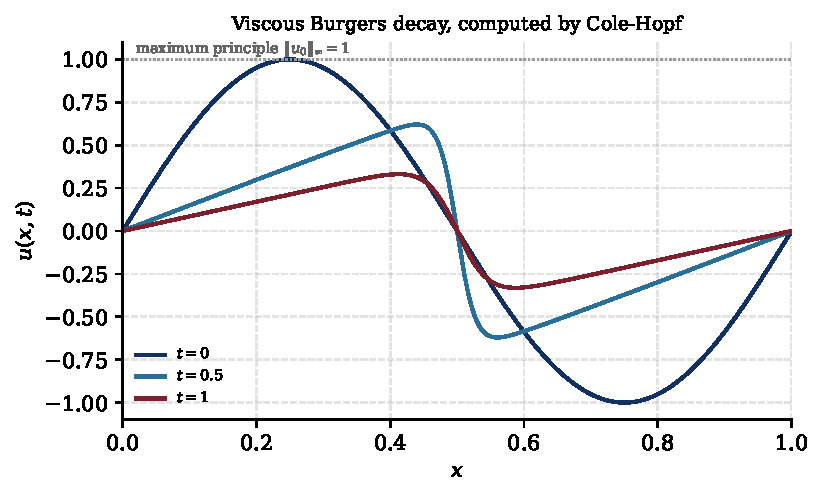
\includegraphics[width=0.80\textwidth]{fig_burgers_exact.pdf}
\caption{\textbf{The Burgers target family, computed exactly.} Viscous Burgers' equation $u_t + u u_x = \nu u_{xx}$ on $[0,1)$ periodic with $\nu = 0.01$ and $u_0(x) = \sin(2\pi x)$, solved by the Cole-Hopf substitution $u = -2\nu\,\partial_x \log \phi$ with $\phi_t = \nu \phi_{xx}$ and $\phi(x,0) = \exp[\cos(2\pi x)/(4\pi\nu)]$. Every trace is computed from the exact solution: the peak falls from $1$ at $t = 0$ to $0.6207$ at $t = 0.5$ and $0.3312$ at $t = 1$, and the profile stays under the maximum-principle bound $\|u_0\|_{\infty} = 1$, drawn as the dotted line. The steepening front near $x \approx 0.5$ is the feature the benchmark scores. Produced by \texttt{figures/make\_figures.py}, which asserts the initial condition, a relative PDE residual and grid independence before writing the file.}
\label{fig:benchmarks}
\end{figure}

% -----------------------------------------------------------------------------
\section{Reference Workflows: What a Benchmark Specification Must Contain}
\label{sec:ch25-protocol}
% -----------------------------------------------------------------------------

Begin with the metric, because it is where the book's two halves meet. All three
benchmarks are scored with the relative $L^{2}$ error
\eqref{eq:rel_l2_loss} of
\chapref{ch:part2-the-practitioner-s-paradigm-infinite-dimen}, the discretized
form of the population risk \eqref{eq:ch01-risk}: the $L^{2}(\Omega)$ norm of the
error divided by the $L^{2}(\Omega)$ norm of the reference field, computed per
sample and then averaged over the batch. The order of those two operations is a
specification choice, not a notational one. A mean of per-sample relative errors
weights a low-amplitude sample as heavily as a high-amplitude one, whereas the
ratio of aggregated norms is dominated by the largest fields in the batch; on a
measure whose amplitude varies by an order of magnitude the two summaries can
differ by a factor of two, and a paper that reports ``relative $L^{2}$ error''
without saying which it used has reported an unidentifiable quantity. Where the
gradient of the field matters more than its energy, as it does for the shock
snapshots below, the honest choice is the inhomogeneous $H^{1}$ functional
\eqref{eq:ch07-sobolev-loss}, which the loss module of
Listing~\ref{lst:ch21-lploss} evaluates once its caller supplies differentiated
fields: one extra differentiation of prediction \emph{and} label, bought for control
of the quantity most applications read.
\index{relative $L^{2}$ error!as benchmark metric}
\index{error metric!per-sample versus batch-aggregated}

Next comes the paired data, and here the arithmetic of amortization from
\eqref{eq:ch01-cost-bookkeeping} becomes concrete. The reference solutions are
produced by classical solvers whose per-query costs are tabulated in
Table~\ref{tab:benchmarks_hardware}: roughly $1.5$ seconds for a finite element
method (FEM) Darcy solve, $4.8$ seconds for a pseudo-spectral Navier--Stokes
trajectory. A thousand training pairs therefore cost about twenty-five minutes of
wall-clock FEM work and eighty minutes of time integration---cheap by simulation
standards, which is why these three problems remain the field's defaults even
though only the Darcy problem arrives in a form an application uses unchanged. The
cost is also a constraint on
honesty: the discretization term in \eqref{eq:ch01-error-split} is invisible if
the reference solver's own resolution is not comfortably finer than the grid on
which the surrogate is trained, since the network is then fitting a solution that
the solver never computed. Record the solver, its spatial and temporal
discretization, its nonlinear and linear tolerances, and the grid on which the
reference was sampled, and sample the reference at least as finely as the finest
evaluation grid the surrogate will see.
\index{pseudo-spectral method!as reference solver}
\index{data generation!reference solver tolerances}

The remaining items of the protocol are short to state and routinely omitted. The
input measure must be given as a measure, not as one representative draw; the
normalization of
\chapref{ch:part2-the-practitioner-s-paradigm-infinite-dimen}---pointwise mean and
standard deviation fields computed over the training ensemble only---must be
frozen before validation data are touched, because normalizing with test
statistics leaks information and inflates accuracy by an amount that grows as the
test set shrinks; and the train/validation/test partition must be reported, an
obligation this chapter discharges by noting that no split ratio is recorded in
what follows, so none of the numbers below should be read as a leaderboard entry.
A single convention worth naming, though none of the numbers below tests it, is
mode-count augmentation: randomly truncating
the retained band below the training maximum should make one checkpoint usable across
several mode budgets, at the price of a slightly worse error at the full budget.
\index{input measure!reporting requirement}
\index{data normalization!frozen before validation}
\index{data augmentation!mode truncation}

Resolution transfer is the protocol item that separates an operator from a
network with a fixed input size, and Part~I states exactly when it is free.
Proposition~\ref{prop:ch06-zeroshot} proves that the spectral branch of a
truncated Fourier neural operator (FNO) returns the identical continuous output,
before the activation, on any grid finer than
$N_{\text{train}} > 2k_{\max}$, provided the input is band-limited within the
retained set $Z_{k_{\max}}$ of \eqref{eq:ch05-modeset}. The hypothesis is the
caveat. None of the three benchmarks below satisfies it: the Burgers target
acquires a shock, the Darcy coefficient field is a rough random function, and the
Navier--Stokes vorticity has a broad spectrum by construction. Super-resolution
results on these problems are therefore measurements, not corollaries, and must be
reported as errors at $N_{\text{test}}$ alongside errors at $N_{\text{train}}$.
\index{resolution transfer!evaluation protocol}
\index{band-limited input!failure on benchmark data}

What, then, distinguishes the three problems? Not size, and not difficulty, but
the term of \eqref{eq:ch05-error-decomposition} each one loads. Darcy flow is an
elliptic coefficient-to-state map that gains derivatives, so its truncation term
decays algebraically in $k_{\max}$ and the theorem applies with its hypotheses
nearly satisfied. Burgers' equation is a parabolic evolution map that also gains
derivatives at fixed $\nu > 0$, but with a constant that deteriorates as the
viscous layer narrows, so the same bound becomes vacuous precisely where the
problem becomes interesting. Navier--Stokes is trained as a one-step map, whereas
applications consume its $K$-fold composition, and the quantity that matters is
the rollout bound \eqref{eq:ch09-gronwall}, whose amplification factor
$\Lambda_{\theta}$ no approximation theorem in this book controls. Three
benchmarks, three different failure modes of one inequality. Figure~\ref{fig:benchmarks}
documents the first two; the third, specified in
Section~\ref{sec:ch25-navierstokes}, comes with no accuracy claim attached,
because none was measured.
\index{benchmark!specification checklist}
\index{benchmark taxonomy}

% -----------------------------------------------------------------------------
\section{Benchmark 1: 1D Viscous Burgers' Equation}
\label{sec:ch25-burgers}
% -----------------------------------------------------------------------------

The 1D viscous Burgers' equation is governed by
\begin{equation}
  \label{eq:ch25-burgers}
  \partial_t u + u \partial_x u = \nu \partial_{xx} u, \qquad x \in [0, 1), \quad t \in [0, 1],
\end{equation}
with periodic boundary conditions. The domain is therefore the torus
$\mathbb{T} = \mathbb{R}/\mathbb{Z}$, not an interval: periodicity is what licenses
the Fourier representation, and it also removes any boundary condition from the
specification, which is why \eqref{eq:ch25-burgers} is the cleanest of the three
tests of discretization invariance. The state is scalar, so the physical input and
output channel counts are both one; the datum is the initial condition $u_0$, and
the target is $u(\cdot, t)$ at one or more times in $[0,1]$. This is a
forward time-evolution operator of the kind introduced in
\eqref{eq:ch03-burgers}, with domain and codomain the same space, in contrast to
the coefficient-to-state map of Section~\ref{sec:ch25-darcy}.

The viscosity is the whole specification. Panel~(a) of Figure~\ref{fig:benchmarks}
is drawn at $\nu = 0.01$, a tenth of the $\nu = 0.1$ of the cited Burgers
experiment \cite{li2021fourier}; its initial trace is consistent with
$u_0(x) = \sin(2\pi x)$, amplitude one. Part~I computes the inviscid gradient
catastrophe for exactly that family: $t_{*} = (2\pi A)^{-1}$, which at $A = 1$ is
$t_{*} \approx 0.16$, occurring where the initial slope is most negative, at
$x = 0.5$. Both snapshots in the panel, $t = 0.5$ and $t = 1.0$, lie well past
that time, so what the reader sees is not steepening in progress but a settled
viscous shock: the $t = 0.5$ trace has developed a sharp descent through zero at
$x \approx 0.5$, and by $t = 1.0$ the descent is confined to a narrow layer with
the smooth remainder of the wave barely changed. The panel is a schematic of the
target family rather than a predicted field, and one feature of it is worth using
as a check on any solver or surrogate. At $\nu > 0$ the maximum principle for
\eqref{eq:ch25-burgers} gives $\sup_x u(\cdot, t) \le \sup_x u_0 = 1$ for all $t$,
yet the $t = 1.0$ trace crests marginally above the initial maximum. A computed
profile that exceeds $\|u_0\|_{L^{\infty}}$ has produced an artifact---an
under-resolved layer, or the ringing of a trigonometric representation near a steep
front---not a feature, and no relative $L^{2}$ number will tell you so.
\index{Burgers equation!benchmark specification}
\index{shock wave!viscous layer width on a grid}
\index{maximum principle!as an implementation check}

Resolution is set by the same layer width. The compressive shock connecting states
$u^{-} > u^{+}$ has the profile \eqref{eq:ch03-shockprofile}, whose transition
layer measures $4\nu/(u^{-} - u^{+})$; writing $\ell_{\nu}$ for that width, at
$\nu = 0.01$ and an order-unity jump $\ell_{\nu} \approx 0.04$ in units of $x$. On
$N = 128$ cells ($\Delta x \approx 7.8 \times 10^{-3}$) the layer spans about five
cells, which is enough for a grid function to represent its shape; on $N = 64$ it
spans two and a
half, which locates the front but no longer resolves the profile, so what the grid
holds is an alias of a shock rather than a shock. That arithmetic, not
a preference for large grids, is why $N = 128$ is the coarsest defensible choice for
this benchmark; it is not the grid of the errors quoted below, which are reported
at $s = 256$ to $s = 8192$ \cite{li2021fourier}. It
also explains the tension Part~I records between accuracy and discontinuity: the
spectral branch represents nothing outside $Z_{k_{\max}}$, so a shock's
$|\hat{u}(k)| = O(|k|^{-1})$ tail is truncated by hypothesis, and the truncation
term of \eqref{eq:ch05-error-decomposition} carries a constant that grows as
$\nu \to 0$.

Tensors and cost follow the layout of
\chapref{ch:part2-the-practitioner-s-paradigm-infinite-dimen}. A batch of initial
conditions arrives as $(B, 1, 128)$; one normalized coordinate channel is
appended---one rather than two, this being a one-dimensional geometry---giving
$(B, 2, 128)$; lifting to width $d_v$ and taking the real FFT along the last axis
gives $(B, d_v, 128, 65)$ complex, of which the two retained blocks at either end
of the spectrum, $(B, d_v, m)$ each, are multiplied by the learned weights. Here $m$
is the retained mode count per band edge---written $m_x, m_y$ in the
two-dimensional tally below, and not to be confused with the $100$ sensor readings of
the DeepONet baseline in Figure~\ref{fig:benchmarks}(b), which the legend also labels
$m$. With
$m = 12$ and $d_v = 32$ the two complex weight tensors hold
$4 m d_v^{2} \approx 4.9 \times 10^{4}$ real numbers per layer, against a
transform cost $\mathcal{O}(d_v N \log N)$ that is essentially flat in $m$: the
one-dimensional benchmark is parameter-cheap and resolution-cheap, which is what
makes it the natural first experiment after Appendix~\ref{app:b}'s heat equation.
\index{tensor layout!benchmark batch shapes}

The number
\chapref{ch:part1-open-theoretical-problems-and-mathematical} interrogates is the
cited paper's own; the book never measured it. The source fixes the
viscosity at $\nu = 0.1$ (Appendix A.3.1) and learns
$u_{0} \mapsto u(\cdot, 1)$, the solution at time one---one output time only
(Section 5.1). Its Table 3 lists relative $L^{2}$ errors
$0.0149$, $0.0158$, $0.0160$, $0.0146$, $0.0142$, $0.0139$ at evaluation
resolutions $s = 256, 512, 1024, 2048, 4096, 8192$; two of the six exceed
$1.5\%$, and no $128$-point Burgers grid appears anywhere in that paper: the
$N = 128$ of the preceding paragraph is this book's own choice, and the two
configurations are distinct. Three qualifications belong to that row, and a
snapshot family would need its own. First, the ambiguity is this book's, not the
source's: the
cited operator ends at $t = 1$, while this section targets $u(\cdot, t)$ at one
or more times, so the reader must still ask whether one model is trained per
$t$, or one model consumes $t$ as an extra input channel, or a one-step map is
iterated to reach $t$; these are three different operators, and the paper does
not say which was trained. Second, each entry of the quoted row compares two
grid functions at the same $s$, the reference subsampled from an $8192$-point
solve (Appendix A.3.1), so it
conflates the approximation and discretization terms of
\eqref{eq:ch01-error-split}. Third, and decisively, the metric is the forgiving
one: as \chapref{ch:part1-open-theoretical-problems-and-mathematical} shows, a
Gibbs overshoot of fixed height on a set of measure $O(1/M)$ contributes
$O(M^{-1/2})$ and a displacement $\delta$ of a unit-height front contributes
$\sqrt{2\delta}$, so a score of $1.4\%$ to $1.6\%$ is fully compatible with a shock placed
in the wrong cell. The benchmark remains the right test---it is the only one of
the three whose target loses regularity---but it should be reported with an
$H^{1}$ or a front-location error beside the $L^{2}$ number.
\index{Burgers equation!snapshot operator ambiguity}

% -----------------------------------------------------------------------------
\section{Benchmark 2: 2D Steady-State Darcy Flow}
\label{sec:ch25-darcy}
% -----------------------------------------------------------------------------

The Darcy flow problem tests an operator's ability to map heterogeneous
coefficient fields to smooth potential solutions:
\begin{equation}
  \label{eq:ch25-darcy}
  -\nabla \cdot \big( K(x) \nabla u(x) \big) = f(x), \qquad x \in [0, 1]^2, \quad u|_{\partial\Omega} = 0.
\end{equation}
Two differences from \eqref{eq:ch25-burgers} matter more than the change of
dimension. The map here is coefficient-to-state: the input is $K$, the output is
$u$, and the spaces differ, so the operator is smoothing rather than
evolutionary---it is the benchmark form of \eqref{eq:darcy}, with the roles of
$a$ and $K$ identified. And the boundary condition is homogeneous Dirichlet on a
square, not periodicity on a torus, which is inconvenient for a spectral
architecture: the Fourier machinery of
\chapref{ch:part2-fourier-neural-operators-fno-from-scratch} is exactly a
representation on $\mathbb{T}^2$, so either the domain is treated as periodic and
the mismatch with $u|_{\partial\Omega} = 0$ is absorbed into the learned map, or
the field is odd-extended. A specification that does not say which has been done
leaves the dominant error term unnamed.

The log-permeability is drawn from a Gaussian random field (GRF), which makes $K$
itself log-normal,
\begin{equation}
  \label{eq:ch25-darcy-measure}
  \log K \sim \mathcal{N}\big(0, (-\Delta + \tau^{2} I)^{-d}\big), \qquad d = 2,
\end{equation}
with $\tau$ a correlation-length parameter and $-\Delta$ the Laplacian with the
problem's own boundary condition \cite{stuart2010inverse}---a Mat\'ern-type
covariance, the standard prior for subsurface coefficients. Read as a covariance
operator, \eqref{eq:ch25-darcy-measure} assigns the mode $k$ a variance of order
$(1 + |k|^{2})^{-2}$, so the sum $\sum_{k} |k|^{2s}(1+|k|^{2})^{-2}$ converges
exactly when $s < 1$ in two dimensions: sample paths of $\log K$ lie in
$H^{s}$ for $s < 1$ and in no better space. Since continuity in two dimensions
requires $s > d/2 = 1$, the coefficient is almost surely unbounded, $K$ is
log-normal rather than essentially bounded, and Assumption~\ref{ass:ellipticity}
fails on the support of the raw measure. This is not a pathology to be tolerated
but a specification to be repaired: draws are truncated into a band
$K \in [K_{\min}, K_{\max}]$ before use, and the band is part of the benchmark,
because the elliptic estimate Part~I derives for \eqref{eq:darcy} is uniform only
over coefficient sets bounded away from zero and from above. Report $K_{\min}$ and
$K_{\max}$ as carefully as the error.
\index{Gaussian random field!Matern-type covariance}
\index{log-normal permeability!truncation and ellipticity}
\index{Darcy flow!benchmark specification}

The regularity that survives is enough to make the benchmark theoretically clean.
With $K$ bounded and measurable, the energy estimate gives $u \in
H^{1}_{0}(\Omega)$; with $K$ smooth, classical regularity lifts the solution to
$H^{2}(\Omega)$. The solution operator therefore has a positive smoothing order
$\alpha$ in the sense of Theorem~\ref{thm:fno_convergence}, its image of a bounded
input set is precompact in $L^{2}$ by Rellich--Kondrachov, and the truncation term
$C_1 k_{\max}^{-\alpha}$ is a live prediction rather than a formality. That is why
\eqref{eq:ch25-darcy} is the default test of the approximation theory and the
default data source for porous-media work \cite{li2021fourier, wen2022ufno}.

Tensor shapes are the two-dimensional case of the tally in
Section~\ref{sec:ch25-burgers}, and larger by the square: a batch arrives as
$(B, 1, 64, 64)$, two coordinate channels make it $(B, 3, 64, 64)$, lifting gives
$(B, d_v, 64, 64)$, and \texttt{torch.fft.rfft2}---the real-to-complex transform
along the two trailing axes---returns $(B, d_v, 64, 33)$ complex, the half-spectrum
being all that conjugate symmetry requires. The two retained corners at
$m_x = m_y = 12$ hold $4 m_x m_y d_v^{2} \approx 5.9 \times 10^{5}$ real numbers
per layer at $d_v = 32$, so four layers carry roughly $2.4$ million spectral
parameters, which is the budget the error floor below buys. The \texttt{einsum}
contracting channels mode by mode is the second term of \eqref{eq:ch8-costs},
$\mathcal{O}(|Z_{k_{\max}}| d_v^{2})$ per
layer, and does not grow with the grid at all; only the transforms do, near-linearly.

No accuracy comparison in this chapter is measured
here; the one it reports is transcribed from the paper that introduced the
benchmark. Table 4 of \cite{li2021fourier} scores the 2-d Darcy problem at four
evaluation resolutions, and FNO returns $0.0108$, $0.0109$, $0.0109$, $0.0098$ at
$s = 85, 141, 211, 421$, against $0.0332$--$0.0369$ for the graph neural operator,
$0.0244$--$0.0259$ for the reduced-basis method and $0.1716$ for a feed-forward
network. Two features of that ordering are architectural rather than matters of
tuning. A convolutional stack aggregates over a receptive field that grows only
with depth, while the pressure at a point of \eqref{eq:ch25-darcy} responds to the
coefficient everywhere --- the long-range coupling Part~I attributes to the Green
kernel --- so its accuracy is limited by distance, not capacity; the fully
convolutional row is the one entry whose error rises monotonically with
resolution, from $0.0253$ to $0.1097$. The FNO's global spectral branch removes the
distance limitation, and its error is essentially flat across the four grids, which
is the resolution-invariance claim of \chapref{ch:part1-discretization-invariance-and-continuum-li}
showing up as an accuracy column rather than as a theorem. What the table does not
settle is the cost of reaching that error: it reports held-out accuracy at four
resolutions and nothing about epochs, hardware or training time, and no
epoch-by-epoch curve for any of these architectures is reproduced in this book.
Multi-scale variants that interleave residual blocks with spectral convolution are
reported to improve precisely this regime on sharper multiphase problems
\cite{wen2022ufno}.
\index{U-Net!as benchmark baseline}
\index{DeepONet!as benchmark baseline}
\index{validation curve!plateau versus divergence}

% -----------------------------------------------------------------------------
\section{Benchmark 3: 2D Incompressible Navier-Stokes Equations}
\label{sec:ch25-navierstokes}
% -----------------------------------------------------------------------------

The 2D incompressible Navier--Stokes equations in vorticity formulation are
\begin{equation}
  \label{eq:ch25-navierstokes}
  \partial_t \omega + \mathbf{u} \cdot \nabla \omega = \nu \Delta \omega + f, \qquad \nabla \cdot \mathbf{u} = 0, \quad \omega = \nabla \times \mathbf{u},
\end{equation}
on the doubly periodic torus $\mathbb{T}^{2} = [0,1)^{2}$. In two dimensions
$\omega$ is the scalar $\partial_1 u_2 - \partial_2 u_1$, and the divergence-free
velocity is recovered from it by the Biot--Savart law
$\mathbf{u} = \nabla^{\perp}(-\Delta_{\mathbb{T}^2})^{-1}\omega$ of
\chapref{ch:part1-partial-differential-equations-as-solution}, so
\eqref{eq:ch25-navierstokes} is a closed equation for one scalar field with no
pressure to eliminate. Periodicity replaces the no-slip condition of a wall-bounded
flow; that single choice is what makes the pseudo-spectral reference solver cheap
and the benchmark standard, and it is also what limits its transfer to
applications, where boundary layers carry the drag. The tensor bookkeeping differs
from Section~\ref{sec:ch25-darcy} in one respect worth stating: the forcing is
fixed and time-independent, so it carries no information across the ensemble and
needs no input channel, and a state enters as $(B, 1, N, N)$ with a single channel
in and out. What the ensemble varies is the initial vorticity---and the viscosity,
if more than one is trained at once, which the paragraph below argues against.

The forcing is Kolmogorov's,
\begin{equation}
  \label{eq:ch25-forcing}
  f(x_1, x_2) = 0.1\big(\sin(2\pi x_2) + \cos(2\pi x_2)\big)
\end{equation}
and the viscosity ranges over $\nu = 10^{-3}$ to $10^{-5}$. Two things about
\eqref{eq:ch25-forcing} must be pinned down before it is used. As written, $f$ is
a scalar added to the vorticity equation,
so it is a vorticity source---the curl of a body force---not a body force; a
specification that reports only ``$f$'' lets the two be confused and changes the
problem's symmetry class. The expression depends on $x_2$ alone and carries
only the wavenumbers $k_2 = \pm 1$, so it injects energy at the largest scale and
drives a shear that the transport term then breaks into smaller scales; its
$L^{2}(\mathbb{T}^2)$ norm is exactly $0.1$, since
$\int_0^1 (\sin 2\pi x_2 + \cos 2\pi x_2)^2\,dx_2 = 1$.
\index{Kolmogorov forcing}
\index{vorticity formulation!forcing as vorticity source}

The viscosity range is the specification's most consequential and least examined
item, and the enstrophy balance \eqref{eq:ch03-enstrophy} prices it. At statistical
steady state the transport term contributes nothing to
$\tfrac{1}{2}\tfrac{d}{dt}\|\omega\|_{L^2}^{2}$, leaving
$\nu\|\nabla\omega\|_{L^2}^{2} = \langle f, \omega\rangle_{L^2}$. Both $\omega$ and
$f$ have zero mean, so the Poincar\'e inequality on $\mathbb{T}^2$ gives
$\|\nabla\omega\|_{L^2}^{2} \ge (2\pi)^{2}\|\omega\|_{L^2}^{2}$, and with
$\langle f,\omega\rangle \le \|f\|_{L^2}\|\omega\|_{L^2} = 0.1\|\omega\|_{L^2}$
\begin{equation}
  \label{eq:ch25-vorticity-bound}
  \|\omega\|_{L^2(\mathbb{T}^2)} \;\le\; \frac{0.1}{(2\pi)^{2}\,\nu}
  \;\approx\; \frac{2.5 \times 10^{-3}}{\nu},
\end{equation}
whence the Biot--Savart law and one more application of Poincar\'e give a velocity
scale of the same order. Equation \eqref{eq:ch25-vorticity-bound} is an a priori
cap rather than a measurement of the realized amplitude, but its
$1/\nu$ dependence is enough to make the point: the three viscosities
$10^{-3}, 10^{-4}, 10^{-5}$ are not three settings of one data distribution but
three distributions with different supports, amplitudes, and spectra. Pooling them
into one training set changes the input measure. Nor is a Reynolds number a
substitute for the viscosity: with the torus as length unit and $U$ of order
unity, $\mathrm{Re} = UL/\nu$ runs from $10^{3}$ to $10^{5}$, yet
\eqref{eq:ch25-vorticity-bound} admits a velocity growing like $1/\nu$, so the
number a reader infers from $\nu$ alone need not be the number the flow has.
Train and score one $\nu$ at a time, and state which.
\index{Reynolds number!convention versus specification}
\index{Navier--Stokes equations!benchmark specification}

The operator being learned is not the solution semigroup of
\eqref{eq:ch25-navierstokes} but a time-$\Delta t$ map, and the neural operator is
trained to map the
vorticity field at time $t$ to $t + \Delta t$, then rolled out recursively across
50 to 100 time steps, where $\omega^{(k)}$ is the surrogate's own iterate and the
step counter $k$ of \eqref{eq:ch25-rollout} is not the wavenumber $k$ used above:
\begin{equation}
  \label{eq:ch25-rollout}
  \omega^{(k+1)} = \mathcal{G}_{\theta}\big(\omega^{(k)}\big),
  \qquad \omega^{(0)} = \omega(\cdot, 0),
  \qquad \text{target: } \omega(\cdot, k\Delta t).
\end{equation}
The input measure is then no longer a prescribed prior at all: it is the empirical
distribution of states visited by the reference trajectory, i.e.\ snapshots drawn
from the attractor of \eqref{eq:ch25-navierstokes}, which is the finite-dimensional
object Part~I's universality discussion appeals to. Three distinct numbers are
conflated in \eqref{eq:ch25-rollout} and all three must be reported: the solver's
own step, small enough to satisfy the Courant--Friedrichs--Lewy (CFL) constraint at
the finest scale present; the interval $\Delta t$ between a training pair's input
and output, an integer multiple of it; and the horizon $K\Delta t$ at which
accuracy is quoted. The rollout is where
the benchmark stops being an approximation problem: the bound
\eqref{eq:ch09-gronwall} amplifies a one-step error $\tau$ by
$\Lambda_{\theta}^{K}$ over $K$ steps, and at $K = 100$ an apparently excellent
one-step surrogate can be worthless. It is also where the single-application cost
read off \eqref{eq:ch8-costs} is incurred $K$ times over in the forward pass, so how
many of those applications carry a gradient is a decision of its own,
taken up in \chapref{ch:part2-training-regimes-optimization-and-failure-}. Nothing
in this chapter measures any of it; the
quantities a Navier--Stokes benchmark should report are the per-step relative
$L^{2}$ error, the horizon at which rollout error first exceeds a stated
threshold, the energy spectrum against the reference, and the discrepancy between
the surrogate's own time-averaged statistics and the solver's. The same structure
reappears at planetary scale in \cite{pathak2022fourcastnet}, and where paired
trajectories are too expensive to sample, the weak-form residual training of the
physics-informed neural operator (PINO) \cite{li2021physics} is the alternative
route to \eqref{eq:ch25-rollout}.
\index{physics-informed neural operator (PINO)!as an alternative to paired data}
\index{autoregressive rollout!error accumulation over 50--100 steps}
\index{one-step map!as learned operator}

\bigskip
\noindent Each of the three specifications above ends at the same place: a number
that comes out of an optimization, not out of an approximation bound. The Darcy
curve in Figure~\ref{fig:benchmarks}(b) flattens, and whether it flattened because
capacity was exhausted or because the schedule had nothing left to give is a
question the specification cannot answer. The Burgers model must be trained at a
viscosity whose target spectrum is barely decaying, which is the regime in which
complex-weighted layers are least forgiving of a step size. The rollout in
\eqref{eq:ch25-rollout} is stable only if the network's own Lipschitz constant
$\Lambda_{\theta}$ stays near one, and no choice of benchmark makes that true by
itself. Those are training questions, and they are the subject of
\chapref{ch:part2-training-regimes-optimization-and-failure-}: the one-cycle
learning-rate schedule and gradient clipping that keep a badly scaled multiplier
array from destabilizing early training, the automatic mixed precision (AMP)
caveat that half-precision transforms under- and overflow on high-dynamic-range
coefficient arrays while \texttt{bfloat16} keeps the single-precision exponent
range, and the pushforward objective that trains a model
on its own unrolled trajectories rather than on teacher-forced inputs. With the
problems fixed, that is what stands between the errors reported here and
reproducible ones.
% -----------------------------------------------------------------------------
